% Aconcagua CFD -- technical report (results of the workflow of ACG-CFD-UG-001)
% Build: make
\documentclass[11pt,a4paper]{article}

\usepackage{fontspec}
\setmainfont{TeX Gyre Pagella}
\setsansfont{TeX Gyre Heros}
\setmonofont{DejaVu Sans Mono}[Scale=0.85]
\usepackage[english]{babel}
\usepackage{amsmath,amssymb}
\usepackage[a4paper,margin=27mm]{geometry}
\usepackage{microtype}
\usepackage[skip=5pt plus 2pt]{parskip}
\usepackage{graphicx}
\usepackage{booktabs,tabularx,array}
\usepackage[table]{xcolor}
\usepackage{titlesec}
\usepackage[numbers,sort&compress]{natbib}
\usepackage[obeyspaces,spaces,hyphens]{url}
\usepackage{xurl}
\usepackage[hidelinks,pdfusetitle]{hyperref}
\usepackage[nameinlink,capitalise,noabbrev]{cleveref}

\definecolor{brand}{HTML}{1F3A5F}
\titleformat*{\section}{\sffamily\bfseries\Large\color{brand}}
\titleformat*{\subsection}{\sffamily\bfseries\large\color{brand}}
\newcommand{\file}{\nolinkurl}
\newcommand{\unit}[2]{#1\,#2}
\newcommand{\yplus}{$y^+$}
\newcolumntype{L}{>{\raggedright\arraybackslash}X}
\renewcommand{\arraystretch}{1.15}

\title{\sffamily\bfseries\color{brand} Drag of the Aconcagua rocket:\\ CFD results and comparison with flight data}
\author{ITBA Rocketry \\ \small Technical report ACG-CFD-TR-001, draft}
\date{2026-10-18}

\begin{document}
\maketitle

\begin{abstract}
The drag coefficient of the Aconcagua sounding rocket was computed with OpenFOAM v2412
on a series of octree meshes, with a pressure-based solver below Mach 1 and a
density-based central-upwind solver above it. The flight of the vehicle at IREC was
reduced to a drag curve with an atmosphere fitted to the GPS and barometric data of the
same flight. On the coarsest mesh, the subsonic drag at zero incidence agrees with the
flight within 2 to 9\,\%, and decreases towards the flight value on the first refined
mesh. The flight shows a transonic drag rise of a factor of two that a semi-empirical
model does not predict. The supersonic computations are not yet converged: the
central-upwind run started from the pressure-based solution shows a growth of the wall
shear stress without limit. This report gives the results; the method is in the user
guide ACG-CFD-UG-001.
\end{abstract}

\section{Introduction}

The aim of the work is the curve $C_D(M, \alpha)$ of the Aconcagua at the conditions of
its flight, with an estimate of the discretization error, for trajectory simulation and
for the comparison of two CFD solvers of different nature (OpenFOAM and Nektar++). The
workflow, its parameters and the reasons for each choice are in the user guide
(\file{flightModel/docs/guide/}). This report gives the results obtained up to
\today{} and the open problems.

\section{Computational setup}

\subsection{Geometry and meshes}

The rocket is \unit{2.955}{m} long with a body diameter $d = \unit{0.151}{m}$, a Von
Kármán nose of \unit{0.8}{m}, a boattail to \unit{0.110}{m}, and four biconvex fins of
constant thickness \unit{11.7}{mm} with \unit{1}{mm} edge radii and \unit{3}{mm} root
fillets. The meshes are half meshes (symmetry plane $z = 0$, fins at $45^\circ$) made by
cutting the full octree mesh. Only \texttt{maxCellSize} changes between meshes, by
$\sqrt{2}$; the layer parameters keep the first cell thickness constant.

\begin{table}[htbp]
\centering
\caption{Meshes.}\label{tab:meshes}
\begin{tabular}{@{}lrrccccc@{}}
\toprule
Mesh & \texttt{maxCellSize} [m] & Cells & Neg.\ vol. & Skewness & Non-orth. & $t_1$ [mm] \\
\midrule
$h_0$ & 2.2627 & 1\,074\,798 & 0 & 2.37 & $65.7^\circ$ & 0.097 \\
$h_1$ & 1.6    & 2\,198\,939 & 0 & 1.72 & $66.0^\circ$ & 0.100 \\
$h_2$ & 1.1314 & 4\,285\,770 & 0 & 1.58 & $65.6^\circ$ & 0.096 \\
$h_3$ & 0.8    & 10\,020\,768 & 0 & 1.41 & $65.9^\circ$ & 0.101 \\
\bottomrule
\end{tabular}
\end{table}

The octree does not refine uniformly: the number of cells grows by 1.95 from $h_1$ to
$h_2$ and by 2.34 from $h_2$ to $h_3$, so the effective refinement ratios are 1.25 and
1.33. The measured first cell is 0.41 times the value of the layer rule, the same on all
meshes, so the rule keeps $t_1$ constant ($y \approx \unit{0.05}{mm}$ at the cell
centre).

\subsection{Solvers and flight conditions}

$M < 1$: \texttt{rhoPimpleFoam} with the transonic pressure equation; $M > 1$:
\texttt{rhoCentralFoam} (Kurganov flux, van Leer reconstruction). Both use local time
stepping, $k$--$\omega$ SST with Spalding wall functions, and air as a perfect gas with
Sutherland viscosity ($Pr = 0.690$ from the Eucken correction). The runs stop when the
1000-iteration moving mean of $C_D$ is within 0.007 of the current value.

The first sweep (\cref{sec:subsonic}) used ISA conditions at the barometric altitude of
the flight. The flight analysis (\cref{sec:flight}) showed an atmosphere about
\unit{20}{K} warmer than ISA; the sweep in progress uses the fitted atmosphere
(\cref{tab:conditions}).

\begin{table}[htbp]
\centering
\caption{Flight conditions: first sweep (ISA) and current sweep (fitted atmosphere).}\label{tab:conditions}
\begin{tabular}{@{}c cc ccc@{}}
\toprule
 & \multicolumn{2}{c}{ISA (first sweep)} & \multicolumn{3}{c}{Fitted atmosphere} \\
\cmidrule(lr){2-3}\cmidrule(l){4-6}
$M$ & $p_\infty$ [Pa] & $T_\infty$ [K] & $t$ [s] & $p_\infty$ [Pa] & $T_\infty$ [K] \\
\midrule
1.8 & 80\,127 & 275.56 & 4.1 & 78\,354 & 295.82 \\
1.2 & 62\,346 & 262.72 & 8.5 & 60\,547 & 280.15 \\
0.8 & 49\,800 & 251.72 & 14.6 & 47\,509 & 266.17 \\
0.6 & 42\,766 & 244.54 & 19.8 & 40\,911 & 257.90 \\
0.3 & 36\,113 & 236.79 & 29.0 & 34\,613 & 248.96 \\
\bottomrule
\end{tabular}
\end{table}

\subsection{Hardware}

Two computers were used: a dual-socket workstation (2 $\times$ Xeon E5-2660 v4, 14 cores
per socket, ECC memory, Open MPI 4.1) and a laptop (Ryzen 7 250, 8 cores, \unit{28}{GB}
without ECC, Open MPI 5.0). The workstation stopped twice under load because of a
defective memory module and is out of service; the runs since 2026-10-15 are on the
laptop. The memory need is about \unit{3}{GB} for each million cells, so $h_3$ does not
fit in the laptop.

\section{Flight data}\label{sec:flight}

\subsection{Atmosphere and speed}

A fit of the hydrostatic profile with a constant lapse rate to 215 pairs of GPS height
and barometric pressure on the descent gives $T_0 = \unit{305.0}{K}$ at the pad
(\unit{896}{m} MSL), a lapse rate of \unit{7.2}{K/km} and $p_0 = \unit{90\,565}{Pa}$,
with an rms error of 0.3\,\% in $\ln p$. The atmosphere was approximately ISA +
\unit{20}{K} from the ground to \unit{8}{km}; individual layers deviate from the fit by
up to \unit{7}{K}.

The speed of the flight computer, integrated, reaches \unit{7837}{m} at apogee against
\unit{8083}{m} from the GPS: it converts pressure to height with ISA and is about
10\,\% low in the coast. The speed was therefore integrated from the axial accelerometer,
anchored at $t = \unit{18}{s}$ to the barometric height with the fitted atmosphere. The
integrated apogee is \unit{8137}{m} (0.7\,\% above the GPS).

\subsection{Drag curve}

\begin{figure}[htbp]
  \centering
  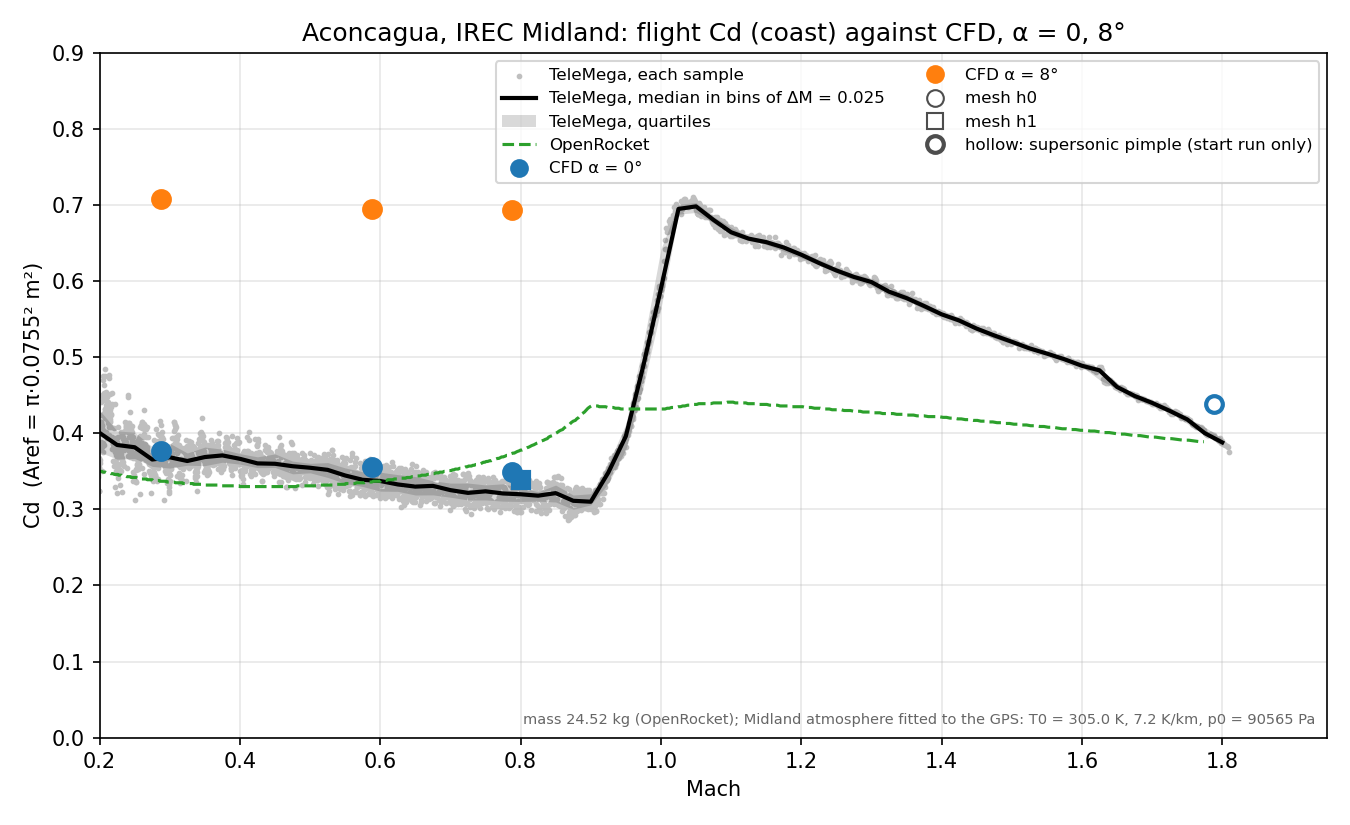
\includegraphics[width=\linewidth]{../../flightData/cdFlight.png}
  \caption{Flight $C_D$ in the coast against the first sweep (ISA conditions) and OpenRocket.}
  \label{fig:cdflight}
\end{figure}

With a post-burnout mass of \unit{24.52}{kg} (OpenRocket), the flight $C_D$ is nearly
constant at 0.32--0.37 below $M = 0.9$, rises to about 0.70 at $M \approx 1.03$, and
decreases to 0.39 at $M = 1.8$ (\cref{fig:cdflight}). OpenRocket follows the subsonic
values but gives only about 0.44 at the transonic peak.

\subsection{Angle of attack}

The vehicle rolled at about 4 revolutions per second in the coast. The mean lateral
acceleration follows $\omega_\text{roll}^2 r$ with $r \approx \unit{2.8}{cm}$ (sensor
off the axis). The component at the roll frequency gives $C_N = 0.01$--$0.03$, that is
$\alpha < 0.2^\circ$ throughout the coast with $C_{N\alpha} \approx \unit{18}{/rad}$.
The angle of $16^\circ$ was therefore removed from the sweep and replaced by $4^\circ$.

\section{Subsonic results}\label{sec:subsonic}

The first sweep ran nine conditions on $h_0$ and one on $h_1$ (ISA conditions).
Coefficients are means over the last 1000 iterations, in wind axes; $C_N$ and $C_A$ are
in body axes.

\begin{table}[htbp]
\centering
\caption{Coefficients of the first sweep.}\label{tab:coeffs}
\begin{tabular}{@{}lccccccc@{}}
\toprule
Run & $C_D$ & $C_L$ & $C_m$ & $C_N$ & $C_A$ & $C_{N\alpha}$ [1/rad] & $x_\text{cp}$ [m] \\
\midrule
M0.3, $0^\circ$, $h_0$ & 0.376 & 0.020 & $-0.38$ & -- & 0.376 & -- & -- \\
M0.6, $0^\circ$, $h_0$ & 0.356 & 0.007 & $-0.14$ & -- & 0.356 & -- & -- \\
M0.8, $0^\circ$, $h_0$ & 0.349 & 0.002 & $-0.03$ & -- & 0.349 & -- & -- \\
M0.8, $0^\circ$, $h_1$ & 0.339 & 0.003 & $-0.06$ & -- & 0.339 & -- & -- \\
M0.3, $8^\circ$, $h_0$ & 0.708 & 2.449 & $-39.6$ & 2.524 & 0.361 & 18.1 & 2.37 \\
M0.6, $8^\circ$, $h_0$ & 0.695 & 2.525 & $-41.1$ & 2.597 & 0.337 & 18.6 & 2.39 \\
M0.8, $8^\circ$, $h_0$ & 0.694 & 2.534 & $-41.3$ & 2.606 & 0.334 & 18.7 & 2.39 \\
M0.3, $16^\circ$, $h_0$ & 1.760 & 5.172 & $-83.2$ & 5.456 & 0.266 & 19.5 & 2.30 \\
M0.6, $16^\circ$, $h_0$ & 1.812 & 5.432 & $-88.2$ & 5.721 & 0.245 & 20.5 & 2.33 \\
M0.8, $16^\circ$, $h_0$ & 1.881 & 5.641 & $-92.1$ & 5.941 & 0.253 & 21.3 & 2.34 \\
\bottomrule
\end{tabular}
\end{table}

\begin{itemize}
\item At zero incidence, $C_D$ is 2 to 9\,\% above the flight (\cref{tab:flight-cfd}),
  and the $h_1$ run is 3\,\% below the $h_0$ run, towards the flight value.
\item The normal-force slope grows with incidence (vortex lift of the body and fins):
  $C_{N\alpha} \approx 18$--$19$ /rad at $8^\circ$, $20$--$21$ /rad at $16^\circ$. The
  centre of pressure is at 15.2--15.8 calibres from the nose, ahead of the fins
  ($x = \unit{2.53}{m}$), and moves forward with incidence.
\item The axial force decreases with incidence ($C_A$ from 0.36 to 0.27 at
  $M = 0.3$); the drag in wind axes rises because of the normal force.
\item $C_L$ at zero incidence is $0.02$ at $M = 0.3$, small but not zero.
\item Mean \yplus{} on the body walls: 2.4 ($M = 0.3$), 5.0 (0.6), 6.9 (0.8); on the
  fins 12 to 33.
\end{itemize}

\begin{table}[htbp]
\centering
\caption{Zero-incidence drag: flight, CFD and OpenRocket.}\label{tab:flight-cfd}
\begin{tabular}{@{}ccccc@{}}
\toprule
$M$ & Flight & CFD & CFD/flight & OpenRocket \\
\midrule
0.3 & 0.369 & 0.376 ($h_0$) & 1.02 & 0.336 \\
0.6 & 0.337 & 0.356 ($h_0$) & 1.05 & 0.337 \\
0.8 & 0.320 & 0.349 ($h_0$), 0.339 ($h_1$) & 1.09, 1.06 & 0.378 \\
1.8 & 0.388 & 0.438 (pimple start run) & 1.13 & 0.389 \\
\bottomrule
\end{tabular}
\end{table}

\section{Supersonic computations}\label{sec:supersonic}

\subsection{Start}

From a uniform free stream, \texttt{rhoCentralFoam} failed at iterations 74 to 256 in
three tests on $h_1$ at $M = 1.8$: the base acts as a piston and empties the region
behind it, and the temperature there falls to zero. \texttt{rhoPimpleFoam}, with a
temperature limit, survives the transient: the base pressure falls to \unit{7900}{Pa}
at iteration 305 and recovers to $p_\text{base}/p_\infty \approx 0.57$ by iteration 755.
A central run started from this solution was stable over its ramp. The supersonic
chains therefore start with a pimple run on the coarsest mesh.

\subsection{Divergence of the central run}

\begin{table}[htbp]
\centering
\caption{Pimple start run against the central run started from it, $h_0$, $M = 1.8$.}\label{tab:central}
\begin{tabular}{@{}lcc@{}}
\toprule
 & Pimple, converged & Central, iteration 550 \\
\midrule
$C_D$ & 0.437 & 0.894, increasing \\
Viscous force, $x$ [N] & 266 & 828 \\
Pressure force, $x$ [N] & 445 & 604 \\
Mean \yplus{} on the body & 16.6 & 33.7 \\
\bottomrule
\end{tabular}
\end{table}

The central run started from the converged pimple solution increased $C_D$ without
limit, mostly through the wall shear stress, which tripled (\cref{tab:central}). The run
was stopped by a hardware failure at iteration 584, not by the solver. The flight value
at this Mach number is 0.39. The cause is open; the candidates are the transfer of the
turbulence fields, the wall treatment of the central template and the limiter at the
wall. Two numerical defects found during this work are corrected: \texttt{mapFields}
can fail with a segmentation fault when source and target are the same mesh, which
earlier went undetected; and under Open MPI 5 the process binding was silently ignored.

\section{Computational cost}

Without suspended intervals, the $h_0$ runs on the laptop cost 20--22\,core-\textmu s
per cell and iteration (\unit{2.7}{s} per iteration with 8 processes), against
\unit{1.77}{s} per iteration with 14 processes on one socket of the workstation. The
laptop is 1.5 times slower per iteration but cheaper per core. The instrumented runs
record CPU cycles, effective clock, IPC and package energy: on $h_0$ with 8 bound
processes the effective clock is \unit{4.4}{GHz} and the IPC about 1, consistent with a
memory-bound solver. These measurements are the basis of the cost comparison with
Nektar++.

\section{Second sweep: fitted atmosphere}\label{sec:sweep2}

The second sweep uses the fitted atmosphere and $\alpha = 0, 4, 8^\circ$, with the
measurement of the computer on each run. \Cref{tab:sweep2} gives the runs that
finished.

\begin{table}[htbp]
\centering
\caption{$C_D$ of the second sweep (mean of the last 1000 iterations).}\label{tab:sweep2}
\begin{tabular}{@{}c ccc c c@{}}
\toprule
$M$ & $0^\circ$, $h_0$ & $4^\circ$, $h_0$ & $8^\circ$, $h_0$ & $0^\circ$, $h_1$ & Flight \\
\midrule
0.3 & 0.383 & 0.462 & 0.713 & 0.352 & 0.369 \\
0.6 & 0.361 & 0.451 & 0.700 & 0.331 & 0.337 \\
0.8 & 0.354 & 0.433 & 0.700 & 0.342 & 0.320 \\
\bottomrule
\end{tabular}
\end{table}

With the real atmosphere, $C_D$ on $h_0$ is 1--2\,\% above the ISA sweep. On $h_1$ it is
3--8\,\% below $h_0$ and within $-5$\,\% to $+7$\,\% of the flight. $m08$-$a08$-$h_1$
gives 0.676.

\paragraph{Failure of the $h_1$ runs at incidence.} Five of the six $h_1$ runs at
$\alpha \neq 0$ stopped at iterations 2 to 7 with a floating point exception in the
turbulence model. A repetition with the computer cold failed at the same iteration, so
the failure is deterministic; a repetition without the mapped \texttt{rDeltaT} failed
too. The cause: 7083 cells of $h_1$ near the fin tips are not inside $h_0$, so
\texttt{mapFields} leaves them with the values of \texttt{0.orig}, and \texttt{0.orig}
has no density field. These cells got $\rho$ equal to the numerical value of
$p_\infty$, about $4\times10^4$, and the first pressure solution reached
$3\times10^9$\,Pa. With \texttt{0/rho} deleted after the mapping, the run continues with
a minimum local time step of $4\times10^{-8}$\,s instead of $2\times10^{-12}$\,s.

\paragraph{Thermal state of the computer.} In the long runs the CPU reached its
\unit{100}{\textdegree C} limit and one memory module \unit{88.5}{\textdegree C}, above
its \unit{85}{\textdegree C} rating. The effective clock varied from 3.5 to
\unit{4.4}{GHz} between runs with the same CPU profile, so the wall time of these runs
is not a comparable cost without the cycle counts.

\section{Reference values for verification}\label{sec:verification}

A replication of the first run of the guide (mesh $h_0$, $M = 0.8$, $\alpha = 0$,
\texttt{pInf} 47\,509\,Pa, \texttt{Tinf} 266.17\,K, \texttt{rhoPimpleFoam}) must give:

\begin{table}[htbp]
\centering
\caption{Reference values of the first run.}\label{tab:verification}
\begin{tabular}{@{}lc@{}}
\toprule
Quantity & Value \\
\midrule
Cells of $h_0$ & 1\,074\,798 \\
Negative cell volumes & 0 \\
$t_1$ on the body walls & \unit{0.097}{mm} \\
$C_D$, mean of the last 1000 iterations & 0.354 \\
Mean \yplus{} on the body walls & 6.2 \\
\bottomrule
\end{tabular}
\end{table}

A difference in $C_D$ larger than the stop tolerance (0.007) shows a different geometry,
mesh or setup. A small difference in the number of cells can come from another
version of cfMesh.

\section{Status and next steps}

\begin{enumerate}
\item The second sweep (\cref{sec:sweep2}): repeat the five $h_1$ runs at incidence
  with the corrected \texttt{Allrun}, then $h_2$; $h_3$ waits for the workstation.
\item Mesh convergence and grid convergence index for $C_D$ at each condition.
\item Diagnosis and correction of the central-run divergence, then the supersonic sweep
  and the transonic drag rise.
\item The same cases with Nektar++, with $h$ and $p$ refinement, and the comparison of
  accuracy against cost.
\end{enumerate}

\bibliographystyle{unsrtnat}
\nocite{toolchain2026,celik2008}
\bibliography{../guide/references}

\end{document}
